\figure{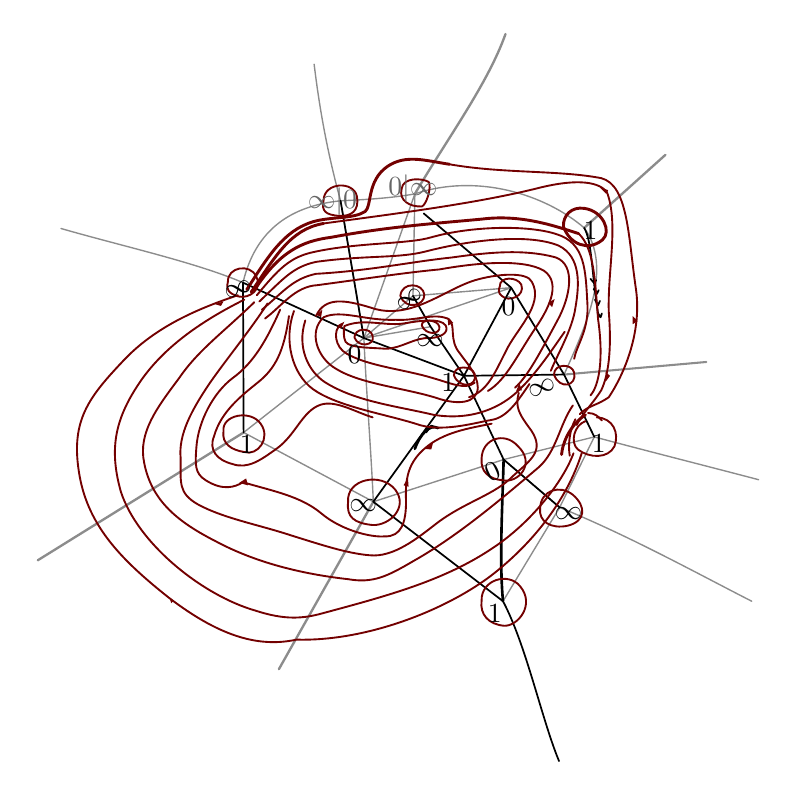
\begin{tikzpicture}[x=0.008cm,y=-0.008cm,line cap=round,line join=round,
  pencil/.style={draw=black!45,line width=0.50pt},
  ink/.style={draw=black,line width=0.62pt},
  redline/.style={draw=red!45!black,line width=0.68pt},
  redheavy/.style={draw=red!45!black,line width=1.05pt}]
\path[use as bounding box] (380,75) rectangle (1560,1250);
% The coordinates below trace the visible strokes. Separate path fragments do
% not assert connections through the dense red junctions at left and right.
% Gray framework and long, blunt-ended exterior rays.
\draw[pencil] (433,394) .. controls (530,422) and (648,448) .. (722,480);
\draw[pencil] (835,133) .. controls (847,233) and (864,302) .. (877,350);
\draw[pencil,line width=0.85pt] (1139,85) .. controls (1111,164) and (1046,252) .. (995,339);
\draw[pencil] (722,480) .. controls (742,395) and (799,358) .. (877,350)
  .. controls (922,348) and (962,345) .. (995,339)
  .. controls (1093,306) and (1201,339) .. (1264,393);
\draw[pencil,line width=0.85pt] (1264,393) -- (1393,277);
\draw[pencil] (995,339) -- (914,568);
\draw[pencil] (995,339) -- (992,501);
\draw[pencil] (877,350) -- (914,568)
  .. controls (918,655) and (926,756) .. (929,828);
\draw[pencil] (914,568) -- (992,501) -- (1148,488);
\draw[pencil] (914,568) -- (1148,488);
\draw[pencil] (914,568) -- (1020,550);
\draw[pencil] (723,718) -- (914,568);
\draw[pencil] (723,718) -- (929,828);
\draw[pencil,line width=0.85pt] (396,921) -- (723,718);
\draw[pencil] (929,828) -- (1136,761) -- (1280,725)
  .. controls (1366,748) and (1473,775) .. (1541,793);
\draw[pencil,line width=0.85pt] (929,828) -- (779,1094);
\draw[pencil] (1136,761) -- (1225,837)
  .. controls (1335,882) and (1442,941) .. (1530,986);
\draw[pencil] (1280,725) -- (1225,837) -- (1135,986);
\draw[pencil] (1264,393) .. controls (1310,457) and (1266,550) .. (1232,626);
\draw[pencil,line width=0.75pt] (1232,626) -- (1458,606);
% Dark retracing within the framework; no heads supplied to the exterior rays.
\draw[ink] (722,480) -- (914,568) -- (1073,628) -- (1232,626);
\draw[ink] (722,480) -- (723,718);
\draw[ink] (877,350) -- (914,568);
\draw[ink] (992,501) -- (1020,550) -- (1073,628) -- (1136,761);
\draw[ink] (1009,370) -- (1148,488) -- (1232,626) -- (1280,725);
\draw[ink] (929,828) -- (1073,628) -- (1148,488);
\draw[ink,line width=0.95pt] (1136,761) .. controls (1134,838) and (1129,922) .. (1135,986);
\draw[ink] (929,828) -- (1135,986)
  .. controls (1172,1056) and (1196,1172) .. (1224,1240);
\draw[ink] (1136,761) -- (1225,837);
\draw[ink] (1264,393) .. controls (1277,416) and (1275,463) .. (1287,535);
% Small hooked/chevron-like black retracings on this descending segment.
\draw[ink] (1274,474) -- (1280,481) -- (1283,476);
\draw[ink] (1279,490) -- (1284,498) -- (1287,492);
\draw[ink] (1281,507) -- (1286,516) -- (1289,509);
\draw[ink] (1285,527) -- (1290,535) -- (1292,529);
\draw[ink,line width=0.95pt] (995,744) .. controls (1003,721) and (1019,704) .. (1032,711);
\draw[ink] (1013,718) -- (1021,707) -- (1032,711);
% Upper red bands, drawn individually rather than as equal parallel bundles.
\draw[redheavy] (728,491) .. controls (761,440) and (786,397) .. (834,383)
  .. controls (862,375) and (898,379) .. (916,367)
  .. controls (927,359) and (918,318) .. (952,295)
  .. controls (981,276) and (1011,286) .. (1050,292);
\draw[redline] (1050,292) .. controls (1135,307) and (1223,301) .. (1291,314)
  .. controls (1334,325) and (1334,408) .. (1346,489)
  .. controls (1356,556) and (1329,623) .. (1303,662)
  .. controls (1285,675) and (1268,676) .. (1257,689);
\draw[redheavy] (735,495) .. controls (773,439) and (797,395) .. (850,386);
\draw[redline] (850,386) .. controls (952,372) and (1090,355) .. (1190,330)
  .. controls (1241,317) and (1284,316) .. (1300,336)
  .. controls (1319,386) and (1301,461) .. (1303,526)
  .. controls (1307,575) and (1305,622) .. (1291,651)
  .. controls (1277,673) and (1264,684) .. (1252,706);
\draw[redheavy] (740,492) .. controls (780,431) and (815,414) .. (862,408)
  .. controls (952,391) and (1028,386) .. (1102,379)
  .. controls (1165,371) and (1220,391) .. (1255,402);
\draw[redline] (1255,402) .. controls (1280,425) and (1281,477) .. (1286,538)
  .. controls (1295,600) and (1288,643) .. (1274,659);
\draw[redline] (744,500) .. controls (778,459) and (796,439) .. (836,431)
  .. controls (905,416) and (984,419) .. (1021,408)
  .. controls (1084,390) and (1175,388) .. (1220,403)
  .. controls (1266,417) and (1266,461) .. (1269,512)
  .. controls (1272,555) and (1252,579) .. (1248,601);
\draw[redline] (748,510) .. controls (786,474) and (801,455) .. (838,447)
  .. controls (918,436) and (969,442) .. (1014,430)
  .. controls (1080,413) and (1173,401) .. (1223,421)
  .. controls (1260,439) and (1256,485) .. (1250,520)
  .. controls (1245,555) and (1220,597) .. (1211,620);
\draw[redline] (752,523) .. controls (785,496) and (800,474) .. (838,466)
  .. controls (925,461) and (987,447) .. (1054,440)
  .. controls (1111,432) and (1168,426) .. (1219,440)
  .. controls (1251,452) and (1242,502) .. (1222,539)
  .. controls (1194,591) and (1175,628) .. (1154,647);
\draw[redline] (757,537) .. controls (783,518) and (804,486) .. (840,484)
  .. controls (922,473) and (980,464) .. (1034,459)
  .. controls (1095,448) and (1168,442) .. (1200,461)
  .. controls (1230,482) and (1204,526) .. (1188,550)
  .. controls (1158,594) and (1140,635) .. (1111,652);
\draw[redline] (838,533) .. controls (852,502) and (884,507) .. (926,520)
  .. controls (988,541) and (1041,491) .. (1091,476)
  .. controls (1125,466) and (1174,462) .. (1181,479)
  .. controls (1201,515) and (1155,555) .. (1139,590)
  .. controls (1122,623) and (1111,652) .. (1081,662);
% Inner turns enclosing the middle vertices.
\draw[redline] (850,535) .. controls (825,558) and (840,600) .. (870,617)
  .. controls (909,641) and (977,647) .. (1029,663)
  .. controls (1063,675) and (1094,672) .. (1095,647)
  .. controls (1095,625) and (1075,605) .. (1067,593)
  .. controls (1048,571) and (1061,548) .. (1049,538)
  .. controls (1026,527) and (998,541) .. (965,539)
  .. controls (916,541) and (878,522) .. (850,535);
\draw[redline] (878,546) .. controls (864,555) and (868,583) .. (887,593)
  .. controls (922,613) and (980,618) .. (1025,632)
  .. controls (1050,639) and (1075,651) .. (1090,639);
\draw[redline] (883,549) .. controls (914,536) and (945,549) .. (976,545)
  .. controls (1001,541) and (1035,535) .. (1044,548)
  .. controls (1050,560) and (1035,567) .. (1020,568)
  .. controls (995,566) and (974,585) .. (948,585)
  .. controls (924,583) and (892,584) .. (885,574)
  .. controls (881,566) and (882,557) .. (883,549);
\draw[redline] (821,540) .. controls (807,583) and (826,621) .. (852,638)
  .. controls (901,669) and (966,676) .. (1025,690)
  .. controls (1088,700) and (1134,677) .. (1161,650)
  .. controls (1190,622) and (1216,582) .. (1233,558);
\draw[redline] (803,525) .. controls (786,571) and (800,625) .. (833,649)
  .. controls (870,676) and (944,688) .. (996,704)
  .. controls (1036,719) and (1088,703) .. (1117,698)
  .. controls (1142,694) and (1159,667) .. (1177,641);
% Long left and lower sweeps. Junctions in the upper-left cluster stay separate.
\draw[redline] (714,500) .. controls (651,521) and (582,550) .. (531,605)
  .. controls (478,661) and (449,698) .. (461,778)
  .. controls (473,862) and (524,917) .. (605,981)
  .. controls (680,1038) and (743,1061) .. (807,1047)
  .. controls (913,1050) and (1037,1004) .. (1114,947)
  .. controls (1182,895) and (1236,826) .. (1260,751);
\draw[redline] (724,507) .. controls (660,539) and (600,579) .. (561,634)
  .. controls (520,693) and (508,741) .. (528,812)
  .. controls (555,895) and (658,977) .. (742,1001)
  .. controls (788,1016) and (817,1014) .. (849,1005)
  .. controls (953,977) and (1042,953) .. (1118,902)
  .. controls (1179,862) and (1230,797) .. (1247,751);
\draw[redline] (740,511) .. controls (693,557) and (651,587) .. (621,631)
  .. controls (586,678) and (555,718) .. (565,766)
  .. controls (577,828) and (620,861) .. (681,892)
  .. controls (749,928) and (826,944) .. (889,951)
  .. controls (929,958) and (952,946) .. (993,922)
  .. controls (1066,881) and (1140,817) .. (1192,773)
  .. controls (1220,748) and (1225,705) .. (1246,675);
\draw[redline] (761,513) .. controls (736,552) and (697,600) .. (671,637)
  .. controls (641,681) and (619,721) .. (623,759)
  .. controls (623,798) and (619,814) .. (650,832)
  .. controls (690,854) and (745,864) .. (797,881)
  .. controls (845,896) and (887,910) .. (923,913)
  .. controls (961,917) and (999,886) .. (1030,862)
  .. controls (1075,828) and (1122,817) .. (1151,787)
  .. controls (1180,761) and (1201,747) .. (1180,715)
  .. controls (1160,688) and (1154,678) .. (1160,655);
\draw[redline] (781,523) .. controls (761,568) and (740,607) .. (705,632)
  .. controls (675,655) and (651,700) .. (648,741)
  .. controls (646,769) and (645,783) .. (663,794)
  .. controls (690,811) and (709,805) .. (722,797)
  .. controls (769,811) and (814,819) .. (847,847)
  .. controls (878,873) and (925,885) .. (947,883)
  .. controls (974,884) and (981,860) .. (981,827)
  .. controls (979,789) and (986,765) .. (1010,744)
  .. controls (1040,717) and (1083,711) .. (1117,704);
\draw[redline] (795,533) .. controls (787,590) and (773,617) .. (745,639)
  .. controls (719,660) and (687,685) .. (676,724)
  .. controls (667,746) and (681,762) .. (705,768)
  .. controls (730,777) and (751,761) .. (775,744)
  .. controls (806,722) and (816,684) .. (845,674)
  .. controls (869,666) and (899,685) .. (928,694);
% Visible separated tails below the right-hand crowded junction.
\draw[redheavy] (1266,690) .. controls (1244,704) and (1230,731) .. (1228,753);
\draw[redline] (1250,697) .. controls (1241,713) and (1238,737) .. (1241,755);
\draw[redline] (1270,687) .. controls (1281,687) and (1287,693) .. (1292,699);
% Small red wedge-like marks, retained as shapes rather than regularized arrows.
\fill[red!45!black] (677,514) -- (691,510) -- (687,517) -- cycle;
\fill[red!45!black] (839,531) -- (848,523) -- (846,535) -- cycle;
\fill[red!45!black] (872,548) -- (883,542) -- (878,553) -- cycle;
\fill[red!45!black] (1047,535) -- (1056,544) -- (1048,548) -- cycle;
\fill[red!45!black] (1289,329) -- (1302,333) -- (1299,339) -- cycle;
\fill[red!45!black] (1341,533) -- (1349,541) -- (1341,546) -- cycle;
\fill[red!45!black] (1298,622) -- (1305,628) -- (1299,636) -- cycle;
\fill[red!45!black] (1207,512) -- (1217,506) -- (1213,519) -- cycle;
\fill[red!45!black] (1156,652) -- (1161,640) -- (1165,651) -- cycle;
\fill[red!45!black] (1011,744) -- (1024,734) -- (1021,745) -- cycle;
\fill[red!45!black] (977,802) -- (984,790) -- (985,804) -- cycle;
\fill[red!45!black] (716,798) -- (727,791) -- (730,802) -- cycle;
\fill[red!45!black] (605,980) -- (612,985) -- (608,989) -- cycle;
% Red rings around the sixteen visible vertices; the N ring remains open.
\draw[redline] (850,349) .. controls (851,320) and (898,318) .. (903,343)
  .. controls (907,366) and (894,375) .. (874,374)
  .. controls (855,372) and (846,368) .. (850,349);
\draw[redline] (974,331) .. controls (976,312) and (1007,314) .. (1017,320)
  .. controls (1022,329) and (1013,357) .. (1006,359)
  .. controls (988,360) and (969,350) .. (974,331);
\draw[redheavy] (1231,391) .. controls (1230,373) and (1244,359) .. (1264,362)
  .. controls (1294,366) and (1308,399) .. (1293,412)
  .. controls (1270,431) and (1241,419) .. (1231,391);
\draw[redline] (698,479) .. controls (697,455) and (733,449) .. (743,470)
  .. controls (754,490) and (732,506) .. (715,502)
  .. controls (698,497) and (695,490) .. (698,479);
\draw[redline] (972,501) .. controls (974,478) and (1008,480) .. (1010,499)
  .. controls (1011,517) and (980,524) .. (972,501);
\draw[redline] (1130,486) .. controls (1129,470) and (1157,470) .. (1164,483)
  .. controls (1171,501) and (1144,512) .. (1133,501)
  .. controls (1127,497) and (1128,490) .. (1130,486);
\draw[redline] (899,567) .. controls (899,552) and (925,550) .. (928,565)
  .. controls (932,580) and (905,584) .. (899,567);
\draw[redline] (1006,548) .. controls (1005,537) and (1031,538) .. (1034,550)
  .. controls (1036,563) and (1012,564) .. (1006,548);
\draw[redline] (1057,627) .. controls (1057,611) and (1085,611) .. (1090,625)
  .. controls (1095,646) and (1065,649) .. (1057,627);
\draw[redline] (1216,626) .. controls (1216,608) and (1245,608) .. (1248,623)
  .. controls (1253,644) and (1225,651) .. (1216,626);
\draw[redline] (691,716) .. controls (688,690) and (734,681) .. (750,704)
  .. controls (767,727) and (745,756) .. (724,749)
  .. controls (704,746) and (688,736) .. (691,716);
\draw[redline] (889,828) .. controls (886,792) and (941,780) .. (964,809)
  .. controls (985,837) and (955,866) .. (928,865)
  .. controls (899,862) and (886,853) .. (889,828);
\draw[redline] (1101,759) .. controls (1102,728) and (1137,716) .. (1158,739)
  .. controls (1189,768) and (1158,799) .. (1135,794)
  .. controls (1112,792) and (1099,780) .. (1101,759);
\draw[redline] (1284,694) .. controls (1310,695) and (1320,719) .. (1312,740)
  .. controls (1302,760) and (1272,759) .. (1254,745)
  .. controls (1241,734) and (1248,706) .. (1266,700);
\draw[redline] (1194,838) .. controls (1195,810) and (1225,800) .. (1246,817)
  .. controls (1268,836) and (1266,859) .. (1238,866)
  .. controls (1211,872) and (1191,859) .. (1194,838);
\draw[redline] (1101,985) .. controls (1100,952) and (1143,939) .. (1162,962)
  .. controls (1187,992) and (1158,1026) .. (1137,1025)
  .. controls (1112,1023) and (1098,1007) .. (1101,985);
% Numerical labels: the first two are pale and crossed by the gray framework.
\node[inner sep=0pt,text=black!60] at (864,352) {$\unsure{\infty|0}$};
\node[inner sep=0pt,text=black!60] at (992,331) {$\unsure{0|\infty}$};
\node[inner sep=0pt] at (1274,398) {$1$};
\node[inner sep=0pt,rotate=20] at (715,490) {$\infty$};
\node[inner sep=0pt,rotate=38] at (987,507) {$\infty$};
\node[inner sep=0pt] at (1144,518) {$0$};
\node[inner sep=0pt] at (899,595) {$0$};
\node[inner sep=0pt] at (1019,572) {$\infty$};
\node[inner sep=0pt] at (1048,638) {$1$};
\node[inner sep=0pt,rotate=22] at (1197,647) {$\infty$};
\node[inner sep=0pt] at (728,738) {$1$};
\node[inner sep=0pt] at (913,834) {$\infty$};
\node[inner sep=0pt,rotate=25] at (1118,780) {$0$};
\node[inner sep=0pt] at (1287,736) {$1$};
\node[inner sep=0pt] at (1239,846) {$\infty$};
\node[inner sep=0pt] at (1122,1005) {$1$};
\end{tikzpicture}}
